\section{Il modello RMM}
Nella progettazione del sistema si sono individuate quattro entità differenti:
\begin{description}
	\item[Concetto teorico] Classe dei concetti musicali prettamente teorici, necessari a una giusta comprensione del mondo musicale. Sono caratterizzati da un titolo (che li identifica) e una descrizione (la quale è ciò che interessa all'utente).
	\item[Strumento] Classe degli strumenti musicali. Sono caratterizzati da un nome (che li identifica) e tutte le informazioni annesse (tra cui una descrizione della struttura dello strumento e le tecniche più comuni).
	\item[Accordo / Tecnica] Classe degli accordi musicali, identificati da un nome, contenenti una descrizione (in termini di note musicali) e degli esempi utili agli utenti. Poiché alcuni strumenti \emph{non} sono polifonici (e non sono quindi in grado di produrre accordi) sono considerate appartenenti a questa classe di oggetti anche le tecniche di utilizzo più avanzate dei suddetti strumenti.
	\item[Quiz] Classe di oggetti che consentono all'utente di ripetere un argomento. Contengono un numero identificativo, una domanda e fino a quattro risposte differenti. Fanno parte di questa classe anche le domande interattive, ovverosia quelle che richiedono all'utente di \textit{``costruire''} una risposta (si considerano aventi una sola risposta possibile).
\end{description}

\subsection{Il modello ER}
\begin{figure}[H]
	\centering
	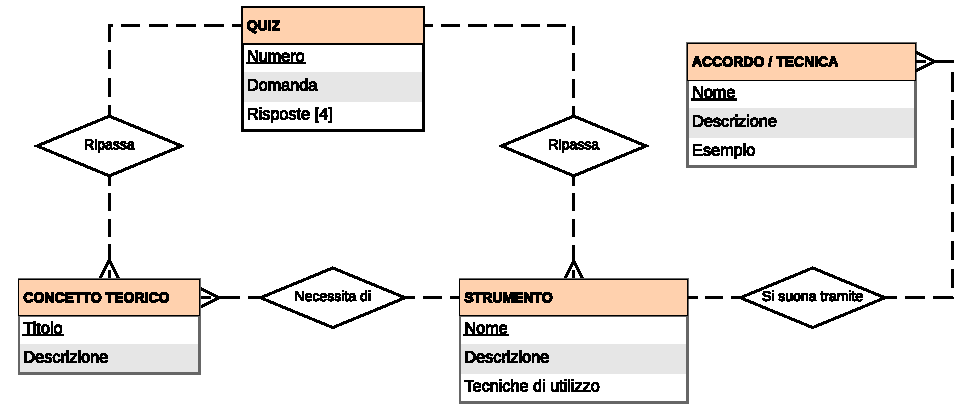
\includegraphics[width=\textwidth]{modello_rmm/modello_er}
	\label{fig:modello-er}
	\caption[Il modello ER di \ProjectTitle{}]{Il modello ER di \ProjectTitle{}. Si noti che la notazione utilizzata prevede le \textit{"chiavi primarie"} sottolineate e i campi multipli scritti con la notazione tipica dell'array (con il numero di ripetizioni racchiuso tra parentesi quadre).}
\end{figure}

\subsection{Progettazione delle slice}
Si sono progettate le \emph{slice} riferite alle quattro entità precedentemente introdotte.

Nei seguenti schemi è indicato con un asterisco ($\ast$) la slice iniziale. Inoltre, sono indicate con delle frecce continue i link che permettono lo spostamento tra le varie slice della stessa entità (su tale freccia è posto il significato del link).

Si noti che nella progettazione delle slice dell'entità \texttt{ACCORDO} non si è inserita alcuna informazione in riferimento alla slice \textit{\texttt{esempio}}: questo poiché la tipologia di esempio e i \textit{media} utilizzati possono variare da strumento a strumento.

Non è visibile ne nei seguenti schemi ne nella progettazione del modello della navigazione la possibilità di suddividere le slice in varie ``schermate'' (a seconda della disponibilità di spazion in relazione ai contenuti), tuttavia si tiene a precisare che è prevista la suddivisione dei contenuti di una stessa slice in più schermate.

\begin{figure}[H]
	\begin{subfigure}[t]{.33\textwidth}
		\centering
		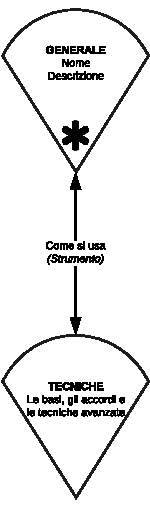
\includegraphics[scale=1]{modello_rmm/slice_strumento}
		\label{fig:slice:strumento}
		\caption{Le \emph{slice} dell'entità \texttt{STRUMENTO}.}
	\end{subfigure}%
	\begin{subfigure}[t]{.66\textwidth}
		\centering
		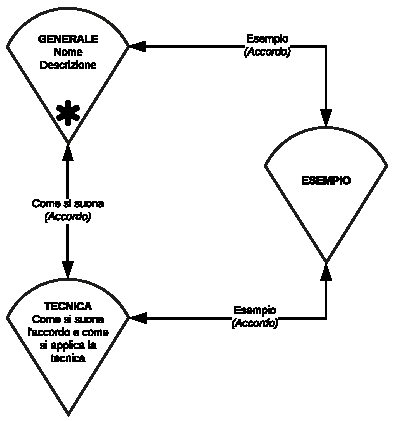
\includegraphics[scale=1]{modello_rmm/slice_accordo}
		\label{fig:slice:accordo}
		\caption{Le \emph{slice} dell'entità \texttt{ACCORDO}.}
	\end{subfigure}
\end{figure}
\begin{figure}[H]\ContinuedFloat
	\begin{subfigure}[t]{.5\textwidth}
		\centering
		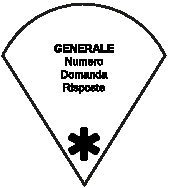
\includegraphics[scale=1]{modello_rmm/slice_quiz}
		\label{fig:slice:quiz}
		\caption{Le \emph{slice} dell'entità \texttt{QUIZ}.}
	\end{subfigure}%
	\begin{subfigure}[t]{.5\textwidth}
		\centering
		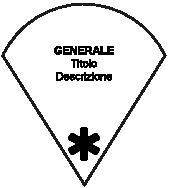
\includegraphics[scale=1]{modello_rmm/slice_concetto_teorico}
		\label{fig:slice:concetto-teorico}
		\caption{Le \emph{slice} dell'entità \texttt{CONCETTO TEORICO}.}
	\end{subfigure}
	\label{fig:slice}
	\caption[Le slice del modello RMM]{Le \emph{slice} del modello RMM di \ProjectTitle{}}
\end{figure}
\subsection{Modello della navigazione}
\begin{figure}[H]
	\centering
	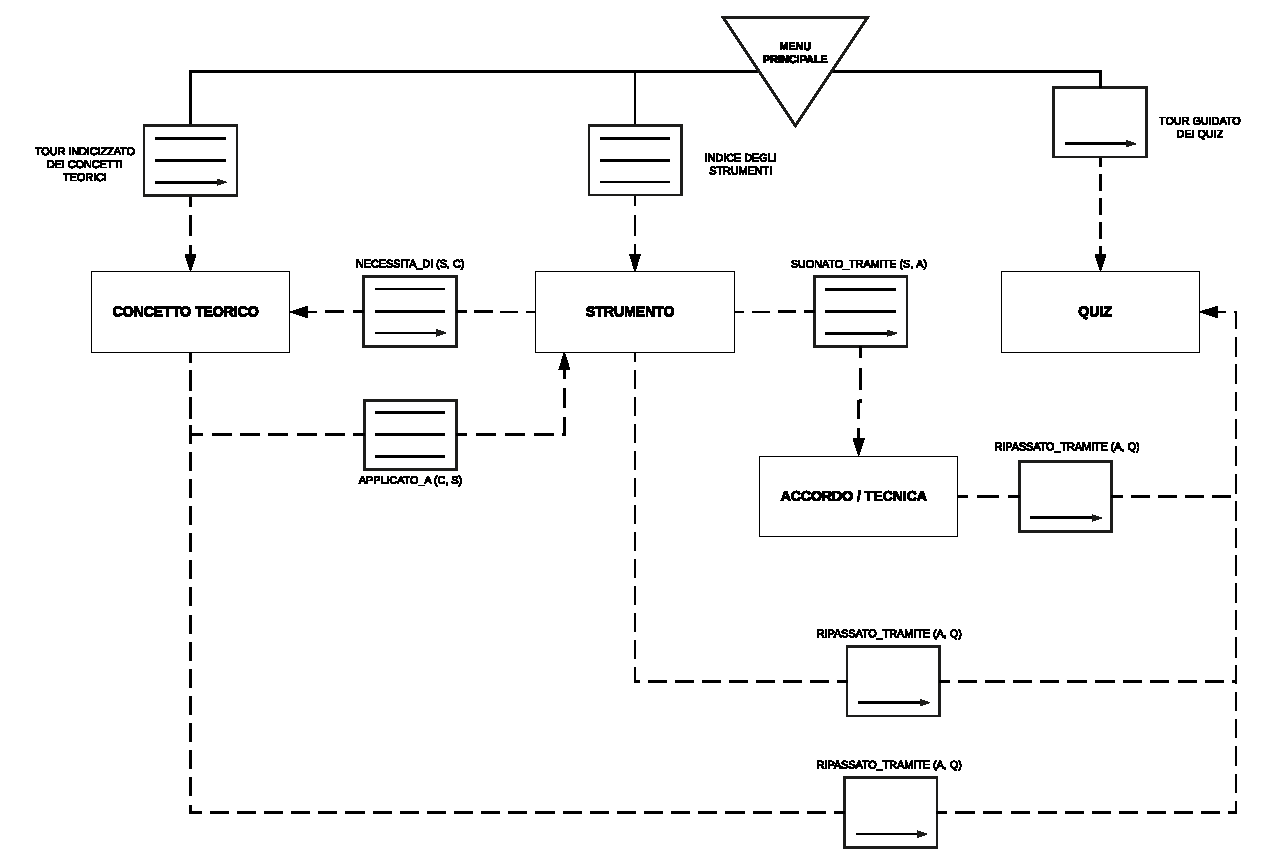
\includegraphics[width=\textwidth]{modello_rmm/navigazione}
	\label{fig:modello-navigazione}
	\caption{Il modello della navigazione di \ProjectTitle{}}
\end{figure}